\documentclass{bioinfo}
\copyrightyear{2013}
\pubyear{2013}

\begin{document}
\firstpage{1}
\title[Gibbs Sampling]{Applications of Gibbs sampling to the Motif Finding Problem}
\author[Alexander Hogue]{Alexander Hogue}
\address{}
\history{}
\editor{}

\maketitle

\begin{abstract}

\section{Motivation:}
The Motif Finding Problem has great relevance to Bioinformatics, indeed, unraveling the mechanisms that regulate gene expression is a major challenge in biology. The probabilistic nature of determining whether a consensus string is indeed the motif lends itself well to the idea of Gibbs Sampling.
\section{Results:}
We provide an efficient, accurate, nondeterministic method for finding motifs. By using an MCMC style sampler, and several tools to discourage convergence to local optima, our implementation locates with a high probability the implanted motif.
\section{Availability:}
The source code to our implementation of the Gibbs Sampler is freely available to view and download online\footnote{https://github.com/defaultnamehere/gibbs-sampler}
\end{abstract}

\section{Introduction}
\subsection{The Motif Finding Problem}

 An important task in understanding gene expression is to identify regulatory elements, especially the binding sites in DNA for transcription factors. These binding sites are short DNA segments that are called motifs. These motifs are of great scientific interest to those doing research in genetics because they correspond to sequences of DNA that control the activation of specific genes. \linebreak \linebreak
In an instance of the motif finding problem, we are given $t$ DNA sequences, each of length $n$, and a length, $l$. Together they form a $t$ by $n$ DNA matrix.
The task is to find sequences of length $l$ in each of the $t$ DNA sequences with maximum "similarity". If each of the sequences shares a common substring, then the Motif Finding Problem reduces to simply finding a substring common to each of the $t$ DNA strings with length $l$. However, in the motif finding problem, we must account for \textit{mutations}. A \textit{mutation} accounts for an index in the motif string which may differ among the corresponding "motifs" in each of the DNA sequences. These occur as motifs may differ slightly from one gene to the next. Further still, the number of these mutations that occur is typically not known \textit{a priori}. 
\linebreak \linebreak
Another complication is the issue of "random" motifs. That is, strings that occur (possibly mutated slightly) in each DNA sequence. As the space of characters DNA strings consist of is small, as the number of DNA strings increase, the probability of a motif being generated by chance increases, especially for small values of $l$ relative to $n$. In these degenerate cases, the motif finding problem loses some meaning.

\section{Approach}
\subsection{Traditional methods of solving the Motif Finding Problem}
Deterministic methods of solving the Motif Finding Problem have had varied success.\citep{Das} As the number of sequences to sample ($t$) and their lengths ($n$) are often large, we seek a more efficient way of finding a motif within several DNA sequences, taking into account mutations. 

Our solution uses Gibbs Sampling, a Markov Chain Monte Carlo (MCMC) approach to probabilistically find the motif. We call the sampler "Markov-Chain", since each step depends only on the previous step; "Monte-Carlo", since we choose the next step non-deterministically. We traverse an $l$-dimensional landscape searching for the global optimum in it, not dissimilar to the classic hill-climbing problem.
\begin{methods}
\section{Methods}
\subsection{The Gibbs Sampler}
Our Gibbs sampler's algorithm is described as follows.
For $t$ DNA samples of length $n$, searching for a motif of length $l$:\\
\begin{enumerate}
    \item Choose $t$ random starting points, one in the first $n - l$ nucleotides of each sequence.
    
    \item While convergence\footnote{See the next section for a discussion on convergence} has not been attained, do 3-6:
    \item Choose a DNA sequence randomly, call it $D$.
    \item Create a \textit{profile} from the $t - 1$ non chosen DNA sequences.
    \item For every starting position in the first $n - l$ positions in $D$, calculate the probability that the $l$-mer starting in each position is generated by the profile. This probability is given by:
        \begin{equation}
            \prod_{i=1}^l P(D[i] \textit{ is at position } i \textit{ in the profile})
        \end{equation}
    Furthermore, these probabilities form a distribution $P$, for each starting position's $l$-mer being generated by the profile.
\item Choose a new starting position (and hence $l$-mer) in $D$ by sampling from $P$. This is equivalent to taking a "step" in one of the $l$ dimensions of our landscape.
\end{enumerate}

We note that in general, traversing an n dimensional space takes exponential time, while Gibbs sampling provides a more efficient approach. The Algorithm performs a random walk in this space, similar to local search. The worst case running time is still the same exponential time, with a pathological (but not necessary to achieve the worst case time) input case being a landscape which is topologically an $l$-dimensional hyperplane\footnote{It's flat.}.
\subsection{Convergence}
The Gibbs Sampler is an algorithm that utilises hill climbing. As is the case with many such algorithms, it is difficult to tell when it has converged. We use the criteria as follows: if the profile has not changed in the last $k$ iterations, we are likely to be at an optima, be it local or global, so we say we have converged. For a given randomly selected staring point, depending on the landscape, it may be likely that we converge to a local optimum. To find the global optimum, we sample from many random starting points, and take the maximum height obtained over all convergences of these starting points. Both $k$ and the number of random starting points are taken as input parameters to the sampler.

\subsection{Implementation}
Our implementation of the Gibbs sampler and its testing program are written in Python 2.7. We recommend running the program with pypy\footnote{\texttt{http://www.pypy.org}}, because hey why not it's faster. \\
We take the several parameters as command line arguments, and refer the reader to the documentation available online\footnote{\texttt{https://github.com/defaultnamehere/gibbs-sampler}}
Implementation details are available as plentiful comments.
\end{methods}


\section{Discussion}
\subsection{Performance}
We conducted tests on our implementation to gauge its performance on a 100*100 DNA matrix, with a motif of length 7 ('GATTACA') to find, with the motif being present in each sample with 0 mutations. The DNA matrix was randomly generated\footnote{See DataGenerator.py}. We present 2 tests in this section. Each test varied one parameter. We calculate the $score$ of a profile as the sum of the most frequent nucleotide in each column of the profile matrix. Figures 1 and 2 show the effects of varying the parameters $k$ and the number of random starting points on the scores ("confidence") of the profiles generated.


\begin{figure}[h]%figure1
    \centerline{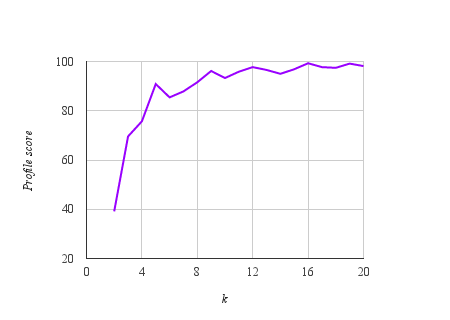
\includegraphics[scale=0.5]{k_score.png}}
\caption{Varying the number of iterations needed to constitute convergence, $k$, shows us unsurprisingly, that the score increases as we demand more consistent results. Note that we fix the number of random starting points at a constant 100 for this experiment.}\label{fig:01}
\end{figure}

\begin{figure}[h]%figure1
    \centerline{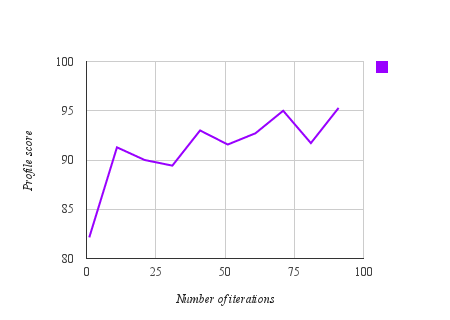
\includegraphics[scale=0.5]{iterations_score.png}}
\caption{We sample from several random starting points and maximise over the values they converge to in an attempt to avoid getting "stuck" in local optima. We see here that as we increase the number of starting points, the chance of finding the global optimum increases, and so the accuracy of the profile increases too. We also note that we fix $k$ at 10 for this experiment. }\label{fig:01}
\end{figure}

We note that when the number of random starting points was 1, the sampler did not converge to the correct motif, even though it was present in the sample. This is to be expected from a randomised algorithm, and indicates that the single random starting point we chose led to convergence to a local optimum.
\subsection{Alternate Metrics for convergence.}
There is discussion on how best to constitute "convergence" for a Gibbs Sampler.
Many accepted local search optimisation techniques can be applied, since the Gibbs Sampler is a variant on local search.\\
There may be merit in using \textit{simulated annealing}, a standard local search technique in which, to avoid becoming stuck in local optima, we probabilistically move away from the optima. \citep{Finkel}

\subsection{Future work}
The alternate methods of convergence may have some merit, and a study comparing them may provide insight regarding their relative efficiencies. In addition, some DNA samples can be biased in their distribution of nucleotides, that is, the distribution of nucleotides is not approximately uniform. In that situation, \textit{relative entropy} can be used to sample without bias. \\
Our implementation allows for infinitely many mutations, and attempts to find the motif under these constraints. We choose to do this since we provide a general approach, and are not looking to solve a specific problem where we know the number of mutations \textit{a priori}. Future work could take the number of mutations we will allow as a parameter. Further, regarding testing, more computing resources would allow for larger DNA matricies to be tested on, which would provide a good oppourtunity to vary the number of mutations in the sample as a parameter, and observe the corresponding profile scores. Finally, we note that we have implemented our sampler in Python. To increase speed on the programming language level, an implementation in C, C++, or Go, possibly involving multithreading could provide a performance increase.


%\bibliographystyle{natbib}
%\bibliographystyle{achemnat}
%\bibliographystyle{plainnat}
%\bibliographystyle{abbrv}
\bibliographystyle{bioinformatics}
%
%\bibliographystyle{plain}
%
%\bibliography{Document}

\begin{thebibliography}{}
\bibitem[Das \textit{et~al}. (2007)]{Das}
    Das \textit{et~al}, "A survey of DNA motif finding algorithms", \textit{Proceedings of the Fourth Annual MCBIOS Conference. Computational Frontiers in Biomedicine} (2007)

\bibitem[Finkel \textit{et~al}. (2005)]{Finkel}
    Finkel, Jenny Rose, Trond Grenager, and Christopher Manning. "Incorporating non-local information into information extraction systems by gibbs sampling." \textit{Proceedings of the 43rd Annual Meeting on Association for Computational Linguistics.} Association for Computational Linguistics (2005)
\end{thebibliography}
\end{document}
